% *****************************************************************************************************
% ****************************                 HW2                     ********************************
% *****************************************************************************************************

% =======================================================
% =======         HEADER FOR DOCUMENT        ============
% =======================================================
    
    % *********  SPECIFIC FOR THIS BOOK  ********
    \def\ProjectAuthorLink{https://github.com/CompilandoConocimiento}
    \def\ProjectNameLink{\ProjectAuthorLink/RandomProject}    
    

    % *********   DOCUMENT ITSELF   **************
    \documentclass[12pt, fleqn]{report}                             %Type of doc and size of font and left equations
    \usepackage[margin=1.2in]{geometry}                             %Margins and Geometry pacakge
    \usepackage{ifthen}                                             %Allow simple programming using if - then
    \usepackage[hidelinks]{hyperref}                                %Allow to create hiperlinks and Fuck Firefox
    \usepackage{pdfpages}                                           %Allow us 'import' PDF's
    \hypersetup{pageanchor=false}                                   %Solve 'double page 1' warnings in build :v
    \setlength{\parindent}{0pt}                                     %Eliminate ugly indentation
    \author{Oscar Andrés Rosas}                                     %Who I am

    % *********   LANGUAJE    *****************
    \usepackage[spanish]{babel}                                     %Please allow me to type in spanish
    \usepackage[utf8]{inputenc}                                     %Lets use UFT-8
    \usepackage[T1]{fontenc}                                        %Allow for better font support
    \usepackage{textcmds}                                           %Allow us to use quoutes
    \usepackage{changepage}                                         %Allow us to use identate paragraphs
    \usepackage{anyfontsize}                                        %All the sizes for fonts wiiiii!

    % *********   MATH AND HIS STYLE  *********
    \usepackage{ntheorem, amsmath, amssymb, amsfonts}               %All fucking math, I want all!
    \usepackage{mathrsfs, mathtools, empheq}                        %All fucking math, I want all!
    \usepackage{cancel}                                             %Negate symbol
    \usepackage{centernot}                                          %Allow me to negate a symbol
    \decimalpoint                                                   %Use decimal point

    % *********   GRAPHICS AND IMAGES *********
    \usepackage{graphicx}                                           %Allow to create graphics
    \usepackage{float}                                              %For images
    \usepackage{wrapfig}                                            %Allow to create images
    \graphicspath{ {Graphics/} }                                    %Where are the images :D

    % *********   LISTS AND TABLES ***********
    \usepackage{listings, listingsutf8}                             %We will be using code here
    \usepackage[inline]{enumitem}                                   %We will need to enumarate
    \usepackage{tasks}                                              %Horizontal lists
    \usepackage{longtable}                                          %Lets make tables awesome
    \usepackage{booktabs}                                           %Lets make tables awesome
    \usepackage{tabularx}                                           %Lets make tables awesome
    \usepackage{multirow}                                           %Lets make tables awesome
    \usepackage{multicol}                                           %Create multicolumns

    % *********   REMOVE SOME ERRORS **********
    \hbadness=10000                                                 %Ignore \vbox and \hbox warings
    \hfuzz=\maxdimen\newdimen\hfuzz                                 %Ignore \vbox and \hbox warings

    % *********   HEADERS AND FOOTERS ********
    \usepackage{fancyhdr}                                           %Lets make awesome headers/footers
    \pagestyle{fancy}                                               %Lets make awesome headers/footers
    \setlength{\headheight}{16pt}                                   %Top line
    \setlength{\parskip}{0.5em}                                     %Top line
    \renewcommand{\footrulewidth}{0.5pt}                            %Bottom line

    \lhead{                                                         %Left Header
        \hyperlink{section.\arabic{section}}                        %Make a link to the current chapter
        {\normalsize{\textsc{\nouppercase{\leftmark}}}}             %And fot it put the name
    }

    \rhead{                                                         %Right Header
        \hyperlink{section.\arabic{section}.\arabic{subsection}}    %Make a link to the current chapter
            {\footnotesize{\textsc{\nouppercase{\rightmark}}}}      %And fot it put the name
    }

    \rfoot{\textsc{\small{Oscar Andres Rosas Hernandez}}}     %This will always be a footer  
    \lfoot{\textsc{\small{Jorge Luís García De Santiago}}}     %This will always be a footer  

    
    
    
% =======================================================
% ===================   COMMANDS    =====================
% =======================================================

    % =========================================
    % =======   NEW ENVIRONMENTS   ============
    % =========================================
    \newenvironment{Indentation}[1][0.75em]                         %Use: \begin{Inde...}[Num]...\end{Inde...}
        {\begin{adjustwidth}{#1}{}}                                 %If you dont put nothing i will use 0.75 em
        {\end{adjustwidth}}                                         %This indentate a paragraph
    
    \newenvironment{SmallIndentation}[1][0.75em]                    %Use: The same that we upper one, just 
        {\begin{adjustwidth}{#1}{}\begin{footnotesize}}             %footnotesize size of letter by default
        {\end{footnotesize}\end{adjustwidth}}                       %that's it
    
    \def \Eq {equation}                                             %Stupid Visual studio error
    \newenvironment{MultiLineEquation}[1]                           %Use: To create MultiLine equations
        {\begin{\Eq}\begin{alignedat}{#1}}                          %Use: \begin{Multi..}{Num. de Columnas}
        {\end{alignedat}\end{\Eq}}                                  %And.. that's it!
    
    \newenvironment{MultiLineEquation*}[1]                          %Use: To create MultiLine equations
        {\begin{\Eq*}\begin{alignedat}{#1}}                         %Use: \begin{Multi..}{Num. de Columnas}
        {\end{alignedat}\end{\Eq*}}                                 %And.. that's it!

    \newenvironment{largeEq} {\begingroup \large}{\endgroup}        %Make eq bigger
    \newenvironment{LargeEq} {\begingroup \Large}{\endgroup}        %Make eq bigger
    \newenvironment{HugeEq} {\begingroup \Huge}{\endgroup}          %Make eq bigger!

    % =========================================
    % == GENERAL TEXT & SYMBOLS ENVIRONMENTS ==
    % =========================================
    
    % =====  TEXT  ======================
    \newcommand \Quote              {\qq}                           %Use: \Quote to use quotes
    \newcommand \Over               {\overline}                     %Use: \Bar to use just for short
    \newcommand \ForceNewLine       {$\Space$\\}                    %Use it in theorems for example
    \newcommand \ForceColumnBreak   {\vfill\null\columnbreak}       %Use only in multicols

    % =====  SPACES  ====================
    \DeclareMathOperator \Space     {\quad}                         %Use: \Space for a cool mega space
    \DeclareMathOperator \MegaSpace {\quad \quad}                   %Use: \MegaSpace for a cool mega mega space
    \DeclareMathOperator \MiniSpace {\;}                            %Use: \Space for a cool mini space
    
    % =====  MATH TEXT  =================
    \newcommand \Such           {\MiniSpace | \MiniSpace}           %Use: \Such like in sets
    \newcommand \Also           {\MiniSpace \text{y} \MiniSpace}    %Use: \Also so it's look cool
    \newcommand \Remember[1]    {\Space\text{\scriptsize{#1}}}      %Use: \Remember so it's look cool
    
    % =====  THEOREMS: IN SPANISH :0  ===
    \newtheorem{Theorem}        {Teorema}[section]                  %Use: \begin{Theorem}[Name]\label{Nombre}...
    \newtheorem{Corollary}      {Colorario}[Theorem]                %Use: \begin{Corollary}[Name]\label{Nombre}...
    \newtheorem{Lemma}[Theorem] {Lemma}                             %Use: \begin{Lemma}[Name]\label{Nombre}...
    \newtheorem{Definition}     {Definición}[section]               %Use: \begin{Definition}[Name]\label{Nombre}...
    \theoremstyle{break}                                            %THEOREMS START 1 SPACE AFTER Fuck!

    % =====  LOGIC  =====================
    \newcommand \lIff    {\leftrightarrow}                          %Use: \lIff for logic iff
    \newcommand \lEqual  {\MiniSpace \Leftrightarrow \MiniSpace}    %Use: \lEqual for a logic double arrow
    \newcommand \lInfire {\MiniSpace \Rightarrow \MiniSpace}        %Use: \lInfire for a logic infire
    \newcommand \lLongTo {\longrightarrow}                          %Use: \lLongTo for a long arrow
    \newcommand \lAnd    {\land}                                    %Use: \lAnd ^
    \newcommand \lOr     {\lor}                                     %Use: \lOr or symbol
    \newcommand \lNot    {\neg}                                     %Use: \lNot for negation

    % =====  FAMOUS SETS  ===============
    \DeclareMathOperator \Naturals     {\mathbb{N}}                 %Use: \Naturals por Notation
    \DeclareMathOperator \Primes       {\mathbb{P}}                 %Use: \Primes por Notation
    \DeclareMathOperator \Integers     {\mathbb{Z}}                 %Use: \Integers por Notation
    \DeclareMathOperator \Racionals    {\mathbb{Q}}                 %Use: \Racionals por Notation
    \DeclareMathOperator \Reals        {\mathbb{R}}                 %Use: \Reals por Notation
    \DeclareMathOperator \Complexs     {\mathbb{C}}                 %Use: \Complex por Notation
    \DeclareMathOperator \GenericField {\mathbb{F}}                 %Use: \GenericField por Notation
    \DeclareMathOperator \VectorSet    {\mathbb{V}}                 %Use: \VectorSet por Notation
    \DeclareMathOperator \SubVectorSet {\mathbb{W}}                 %Use: \SubVectorSet por Notation
    \DeclareMathOperator \Polynomials  {\mathbb{P}}                 %Use: \Polynomials por Notation
    \DeclareMathOperator \VectorSpace  {\VectorSet_{\GenericField}} %Use: \VectorSpace por Notation
    \DeclareMathOperator \LinealTransformation {\mathcal{T}}        %Use: \LinealTransformation for a cool T
    \DeclareMathOperator \LinTrans      {\mathcal{T}}               %Use: \LinTrans for a cool T
    \DeclareMathOperator \Laplace       {\mathcal{L}}               %Use: \LinTrans for a cool T

    % =====  CONTAINERS   ===============
    \newcommand{\Set}[1]            {\left\{ \; #1 \; \right\}}     %Use: \Set {Info} for INTELLIGENT space 
    \newcommand{\bigSet}[1]         {\big\{  \; #1 \; \big\}}       %Use: \bigSet  {Info} for space 
    \newcommand{\BigSet}[1]         {\Big\{  \; #1 \; \Big\}}       %Use: \BigSet  {Info} for space 
    \newcommand{\biggSet}[1]        {\bigg\{ \; #1 \; \bigg\}}      %Use: \biggSet {Info} for space 
    \newcommand{\BiggSet}[1]        {\Bigg\{ \; #1 \; \Bigg\}}      %Use: \BiggSet {Info} for space 
        
    \newcommand{\Wrap}[1]           {\left( #1 \right)}             %Use: \Wrap {Info} for INTELLIGENT space
    \newcommand{\bigWrap}[1]        {\big( \; #1 \; \big)}          %Use: \bigBrackets  {Info} for space 
    \newcommand{\BigWrap}[1]        {\Big( \; #1 \; \Big)}          %Use: \BigBrackets  {Info} for space 
    \newcommand{\biggWrap}[1]       {\bigg( \; #1 \; \bigg)}        %Use: \biggBrackets {Info} for space 
    \newcommand{\BiggWrap}[1]       {\Bigg( \; #1 \; \Bigg)}        %Use: \BiggBrackets {Info} for space 

    \newcommand{\Brackets}[1]       {\left[ #1 \right]}             %Use: \Brackets {Info} for INTELLIGENT space
    \newcommand{\bigBrackets}[1]    {\big[ \; #1 \; \big]}          %Use: \bigBrackets  {Info} for space 
    \newcommand{\BigBrackets}[1]    {\Big[ \; #1 \; \Big]}          %Use: \BigBrackets  {Info} for space 
    \newcommand{\biggBrackets}[1]   {\bigg[ \; #1 \; \bigg]}        %Use: \biggBrackets {Info} for space 
    \newcommand{\BiggBrackets}[1]   {\Bigg[ \; #1 \; \Bigg]}        %Use: \BiggBrackets {Info} for space 

    \newcommand{\Generate}[1]   {\left\langle #1 \right\rangle}     %Use: \Generate {Info} <>
    \newcommand{\Floor}[1]      {\left \lfloor #1 \right \rfloor}   %Use: \Floor {Info} for floor 
    \newcommand{\Ceil}[1]       {\left \lceil #1 \right \rceil }    %Use: \Ceil {Info} for ceil
    
    % =====  BETTERS MATH COMMANDS   =====
    \newcommand{\pfrac}[2]      {\Wrap{\dfrac{#1}{#2}}}             %Use: Put fractions in parentesis
    \newcommand{\Sum}           {\displaystyle \sum}                %Use: Sum to big sum
    \newcommand{\Int}           {\displaystyle \int}                %Use: Sum to big integral


    % =========================================
    % ====   LINEAL ALGEBRA & VECTORS    ======
    % =========================================

    % ===== UNIT VECTORS  ================
    \newcommand{\hati}      {\hat{\imath}}                           %Use: \hati for unit vector    
    \newcommand{\hatj}      {\hat{\jmath}}                           %Use: \hatj for unit vector    
    \newcommand{\hatk}      {\hat{k}}                                %Use: \hatk for unit vector

    % ===== MAGNITUDE  ===================
    \newcommand{\abs}[1]    {\left\lvert #1 \right\lvert}           %Use: \abs{expression} for |x|
    \newcommand{\Abs}[1]    {\left\lVert #1 \right\lVert}           %Use: \Abs{expression} for ||x||
    \newcommand{\Mag}[1]    {\left| #1 \right|}                     %Use: \Mag {Info} 
    
    \newcommand{\bVec}[1]   {\mathbf{#1}}                           %Use for bold type of vector
    \newcommand{\lVec}[1]   {\overrightarrow{#1}}                   %Use for a long arrow over a vector
    \newcommand{\uVec}[1]   {\mathbf{\hat{#1}}}                     %Use: Unitary Vector Example: $\uVec{i}

    % ===== FN LINEAL TRANSFORMATION  ====
    \newcommand{\FnLinTrans}[1]{\mathcal{T}\Wrap{#1}}               %Use: \FnLinTrans for a cool T
    \newcommand{\VecLinTrans}[1]{\mathcal{T}\pVector{#1}}           %Use: \LinTrans for a cool T
    \newcommand{\FnLinealTransformation}[1]{\mathcal{T}\Wrap{#1}}   %Use: \FnLinealTransformation

    % ===== ALL FOR DOT PRODUCT  =========
    \makeatletter                                                   %WTF! IS THIS
    \newcommand*\dotP{\mathpalette\dotP@{.5}}                       %Use: \dotP for dot product
    \newcommand*\dotP@[2] {\mathbin {                               %WTF! IS THIS            
        \vcenter{\hbox{\scalebox{#2}{$\m@th#1\bullet$}}}}           %WTF! IS THIS
    }                                                               %WTF! IS THIS
    \makeatother                                                    %WTF! IS THIS

    % === WRAPPERS FOR COLUMN VECTOR ===
    \newcommand{\pVector}[1]                                        %Use: \pVector {Matrix Notation} use parentesis
        { \ensuremath{\begin{pmatrix}#1\end{pmatrix}} }             %Example: \pVector{a\\b\\c} or \pVector{a&b&c} 
    \newcommand{\lVector}[1]                                        %Use: \lVector {Matrix Notation} use a abs 
        { \ensuremath{\begin{vmatrix}#1\end{vmatrix}} }             %Example: \lVector{a\\b\\c} or \lVector{a&b&c} 
    \newcommand{\bVector}[1]                                        %Use: \bVector {Matrix Notation} use a brackets 
        { \ensuremath{\begin{bmatrix}#1\end{bmatrix}} }             %Example: \bVector{a\\b\\c} or \bVector{a&b&c} 
    \newcommand{\Vector}[1]                                         %Use: \Vector {Matrix Notation} no parentesis
        { \ensuremath{\begin{matrix}#1\end{matrix}} }               %Example: \Vector{a\\b\\c} or \Vector{a&b&c}

    % === MAKE MATRIX BETTER  =========
    \makeatletter                                                   %Example: \begin{matrix}[cc|c]
    \renewcommand*\env@matrix[1][*\c@MaxMatrixCols c] {             %WTF! IS THIS
        \hskip -\arraycolsep                                        %WTF! IS THIS
        \let\@ifnextchar\new@ifnextchar                             %WTF! IS THIS
        \array{#1}                                                  %WTF! IS THIS
    }                                                               %WTF! IS THIS
    \makeatother                                                    %WTF! IS THIS
    
    \newcommand{\adotP}[2] {\left< #1, #2 \right> }                 %Use for <x, y>
    \newcommand{\wdotP}[2] {\Wrap{ #1, #2 } }                       %Use for (x, y)
    \newcommand{\cdotP}[2] {\Wrap{ #1 \dotP #2 } }                  %Use for (x * y)


    % =========================================
    % =======   FAMOUS FUNCTIONS   ============
    % =========================================

    % == TRIGONOMETRIC FUNCTIONS  ====
    \newcommand{\Cos}[1] {\cos\Wrap{#1}}                            %Simple wrappers
    \newcommand{\Sin}[1] {\sin\Wrap{#1}}                            %Simple wrappers
    \newcommand{\Tan}[1] {tan\Wrap{#1}}                             %Simple wrappers
    
    \newcommand{\Sec}[1] {sec\Wrap{#1}}                             %Simple wrappers
    \newcommand{\Csc}[1] {csc\Wrap{#1}}                             %Simple wrappers
    \newcommand{\Cot}[1] {cot\Wrap{#1}}                             %Simple wrappers

    % === COMPLEX ANALYSIS TRIG ======
    \newcommand \Cis[1]  {\Cos{#1} + i \Sin{#1}}                    %Use: \Cis for cos(x) + i sin(x)
    \newcommand \pCis[1] {\Wrap{\Cis{#1}}}                          %Use: \pCis for the same with parantesis
    \newcommand \bCis[1] {\Brackets{\Cis{#1}}}                      %Use: \bCis for the same with Brackets


    % =========================================
    % ===========     CALCULUS     ============
    % =========================================

    % ====== TRANSFORMS =============
    \newcommand{\FourierT}[1]   {\mathscr{F} \left\{ #1 \right\} }  %Use: \FourierT {Funtion}
    \newcommand{\InvFourierT}[1]{\mathscr{F}^{-1}\left\{#1\right\}} %Use: \InvFourierT {Funtion}

    % ====== DERIVATIVES ============
    \newcommand \MiniDerivate[1][x]   {\dfrac{d}{d #1}}             %Use: \MiniDerivate[var] for simple use [var]
    \newcommand \Derivate[2]          {\dfrac{d \; #1}{d #2}}       %Use: \Derivate [f(x)][x]
    \newcommand \MiniUpperDerivate[2] {\dfrac{d^{#2}}{d#1^{#2}}}    %Mini Derivate High Orden Derivate -- [x][pow]
    \newcommand \UpperDerivate[3] {\dfrac{d^{#3} \; #1}{d#2^{#3}}}  %Complete High Orden Derivate -- [f(x)][x][pow]
    
    \newcommand \MiniPartial[1][x] {\dfrac{\partial}{\partial #1}}  %Use: \MiniDerivate for simple use [var]
    \newcommand \Partial[2] {\dfrac{\partial \; #1}{\partial #2}}   %Complete Partial Derivate -- [f(x)][x]
    \newcommand \MiniUpperPartial[2]                                %Mini Derivate High Orden Derivate -- [x][pow] 
        {\dfrac{\partial^{#2}}{\partial #1^{#2}}}                   %Mini Derivate High Orden Derivate
    \newcommand \UpperPartial[3]                                    %Complete High Orden Derivate -- [f(x)][x][pow]
        {\dfrac{\partial^{#3} \; #1}{\partial#2^{#3}}}              %Use: \UpperDerivate for simple use

    \DeclareMathOperator \Evaluate  {\Big|}                         %Use: \Evaluate por Notation

    % ====== INTEGRALS ============
    \newcommand{\inftyInt} {\int_{-\infty}^{\infty}}                %Use: \inftyInt for simple integrants
    
        
% =======================================================
% ===========      COLOR: MATERIAL DESIGN     ===========
% =======================================================

    % =====  COLORS ==================
    \definecolor{RedMD}{HTML}{F44336}                               %Use: Color :D        
    \definecolor{Red100MD}{HTML}{FFCDD2}                            %Use: Color :D        
    \definecolor{Red200MD}{HTML}{EF9A9A}                            %Use: Color :D        
    \definecolor{Red300MD}{HTML}{E57373}                            %Use: Color :D        
    \definecolor{Red700MD}{HTML}{D32F2F}                            %Use: Color :D 

    \definecolor{PurpleMD}{HTML}{9C27B0}                            %Use: Color :D        
    \definecolor{Purple100MD}{HTML}{E1BEE7}                         %Use: Color :D        
    \definecolor{Purple200MD}{HTML}{EF9A9A}                         %Use: Color :D        
    \definecolor{Purple300MD}{HTML}{BA68C8}                         %Use: Color :D        
    \definecolor{Purple700MD}{HTML}{7B1FA2}                         %Use: Color :D 

    \definecolor{IndigoMD}{HTML}{3F51B5}                            %Use: Color :D        
    \definecolor{Indigo100MD}{HTML}{C5CAE9}                         %Use: Color :D        
    \definecolor{Indigo200MD}{HTML}{9FA8DA}                         %Use: Color :D        
    \definecolor{Indigo300MD}{HTML}{7986CB}                         %Use: Color :D        
    \definecolor{Indigo700MD}{HTML}{303F9F}                         %Use: Color :D 

    \definecolor{BlueMD}{HTML}{2196F3}                              %Use: Color :D        
    \definecolor{Blue100MD}{HTML}{BBDEFB}                           %Use: Color :D        
    \definecolor{Blue200MD}{HTML}{90CAF9}                           %Use: Color :D        
    \definecolor{Blue300MD}{HTML}{64B5F6}                           %Use: Color :D        
    \definecolor{Blue700MD}{HTML}{1976D2}                           %Use: Color :D        
    \definecolor{Blue900MD}{HTML}{0D47A1}                           %Use: Color :D  

    \definecolor{CyanMD}{HTML}{00BCD4}                              %Use: Color :D        
    \definecolor{Cyan100MD}{HTML}{B2EBF2}                           %Use: Color :D        
    \definecolor{Cyan200MD}{HTML}{80DEEA}                           %Use: Color :D        
    \definecolor{Cyan300MD}{HTML}{4DD0E1}                           %Use: Color :D        
    \definecolor{Cyan700MD}{HTML}{0097A7}                           %Use: Color :D        
    \definecolor{Cyan900MD}{HTML}{006064}                           %Use: Color :D 

    \definecolor{TealMD}{HTML}{009688}                              %Use: Color :D        
    \definecolor{Teal100MD}{HTML}{B2DFDB}                           %Use: Color :D        
    \definecolor{Teal200MD}{HTML}{80CBC4}                           %Use: Color :D        
    \definecolor{Teal300MD}{HTML}{4DB6AC}                           %Use: Color :D        
    \definecolor{Teal700MD}{HTML}{00796B}                           %Use: Color :D        
    \definecolor{Teal900MD}{HTML}{004D40}                           %Use: Color :D 

    \definecolor{GreenMD}{HTML}{4CAF50}                             %Use: Color :D        
    \definecolor{Green100MD}{HTML}{C8E6C9}                          %Use: Color :D        
    \definecolor{Green200MD}{HTML}{A5D6A7}                          %Use: Color :D        
    \definecolor{Green300MD}{HTML}{81C784}                          %Use: Color :D        
    \definecolor{Green700MD}{HTML}{388E3C}                          %Use: Color :D        
    \definecolor{Green900MD}{HTML}{1B5E20}                          %Use: Color :D

    \definecolor{AmberMD}{HTML}{FFC107}                             %Use: Color :D        
    \definecolor{Amber100MD}{HTML}{FFECB3}                          %Use: Color :D        
    \definecolor{Amber200MD}{HTML}{FFE082}                          %Use: Color :D        
    \definecolor{Amber300MD}{HTML}{FFD54F}                          %Use: Color :D        
    \definecolor{Amber700MD}{HTML}{FFA000}                          %Use: Color :D        
    \definecolor{Amber900MD}{HTML}{FF6F00}                          %Use: Color :D

    \definecolor{OrangeMD}{HTML}{ff9800}                            %Use: Color :D        
    \definecolor{Orange100MD}{HTML}{ffe0b2}                         %Use: Color :D        
    \definecolor{Orange200MD}{HTML}{ffcc80}                         %Use: Color :D        
    \definecolor{Orange300MD}{HTML}{ffb74d}                         %Use: Color :D        
    \definecolor{Orange700MD}{HTML}{fb8c00}                         %Use: Color :D        
    \definecolor{Orange900MD}{HTML}{ef6c00}                         %Use: Color :D

    \definecolor{BlueGreyMD}{HTML}{607D8B}                          %Use: Color :D        
    \definecolor{BlueGrey100MD}{HTML}{CFD8DC}                       %Use: Color :D        
    \definecolor{BlueGrey200MD}{HTML}{B0BEC5}                       %Use: Color :D        
    \definecolor{BlueGrey300MD}{HTML}{90A4AE}                       %Use: Color :D        
    \definecolor{BlueGrey700MD}{HTML}{455A64}                       %Use: Color :D        
    \definecolor{BlueGrey900MD}{HTML}{263238}                       %Use: Color :D        

    \definecolor{DeepPurpleMD}{HTML}{673AB7}                        %Use: Color :D

    \definecolor{SolarizedBase}{HTML}{fdf6e3}                       %Use: Color :D
    \definecolor{SolarizedFont}{HTML}{073642}                       %Use: Color :D

    % =====  ENVIRONMENT ==============
    \newcommand{\Color}[2]{\textcolor{#1}{#2}}                      %Simple color environment
    \newenvironment{ColorText}[1]                                   %Use: \begin{ColorText}
        { \leavevmode\color{#1}\ignorespaces }                      %That's is!


% =======================================================
% ===========           CODE EDITING          ===========
% =======================================================

    \newcommand{\fontCode}        { \ttfamily\bfseries }            %Use: \fontCode for font
    \newcommand{\fontCodeTiny}    { \fontCode\tiny }                %Sizes
    \newcommand{\fontCodeFoot}    { \fontCode\footnotesize }        %Sizes
    \newcommand{\fontCodeScript}  { \fontCode\scriptsize }          %Sizes
    \newcommand{\fontCodeCostume} { \fontCode\fontsize{10}{7} }     %Sizes
   

    % =====  CODE EDITOR =============
    \lstdefinestyle{CompilandoStyle} {                              %This is Code Style
        backgroundcolor     = \color{BlueGrey900MD},                %Background Color  
        basicstyle          = \fontCodeTiny\color{white},           %Style of text
        commentstyle        = \color{BlueGrey200MD},                %Comment style
        stringstyle         = \color{Green300MD},                   %String style
        keywordstyle        = \color{Blue300MD},                    %keywords style
        numberstyle         = \tiny\color{TealMD},                  %Size of a number
        frame               = none,                                 %Adds a frame around the code
        breakatwhitespace   = true,                                 %Style   
        breaklines          = true,                                 %Style   
        showstringspaces    = false,                                %Hate those spaces                  
        breaklines          = true,                                 %Style                   
        keepspaces          = true,                                 %Style                   
        numbers             = left,                                 %Style                   
        numbersep           = 10pt,                                 %Style 
        xleftmargin         = \parindent,                           %Style 
        tabsize             = 4,                                    %Style
        inputencoding       = utf8/latin1                           %Allow me to use special chars
    }

    % =====  CODE EDITOR =============
    \lstdefinestyle{CompilandoStylePurity} {                        %This is Code Style
        backgroundcolor     = \color{white},                        %Background Color  
        basicstyle          = \fontCodeTiny\color{BlueGrey900MD},   %Style of text
        commentstyle        = \color{Green300MD},                   %Comment style
        stringstyle         = \color{Teal700MD},                    %String style
        keywordstyle        = \color{Blue700MD},                    %keywords style
        numberstyle         = \tiny\color{TealMD},                  %Size of a number
        frame               = none,                                 %Adds a frame around the code
        breakatwhitespace   = true,                                 %Style   
        breaklines          = true,                                 %Style   
        showstringspaces    = false,                                %Hate those spaces                  
        breaklines          = true,                                 %Style                   
        keepspaces          = true,                                 %Style                   
        numbers             = left,                                 %Style                   
        numbersep           = 11pt,                                 %Style 
        xleftmargin         = \parindent,                           %Style 
        tabsize             = 4,                                    %Style
        inputencoding       = utf8/latin1                           %Allow me to use special chars
    }

    % =====  CODE EDITOR =============
    \lstdefinestyle{CompilandoStyleSolarized} {                     %This is Code Style
        backgroundcolor     = \color{SolarizedBase},                %Background Color  
        basicstyle          = \fontCodeFoot\color{SolarizedFont},   %Style of text
        commentstyle        = \color{Green300MD},                   %Comment style
        stringstyle         = \color{Teal700MD},                    %String style
        keywordstyle        = \color{Blue700MD},                    %keywords style
        numberstyle         = \tiny\color{TealMD},                  %Size of a number
        frame               = none,                                 %Adds a frame around the code
        breakatwhitespace   = true,                                 %Style   
        breaklines          = true,                                 %Style   
        showstringspaces    = false,                                %Hate those spaces                  
        breaklines          = true,                                 %Style                   
        keepspaces          = true,                                 %Style                   
        numbers             = none,                                 %Style                   
        tabsize             = 4,                                    %Style
        inputencoding       = utf8/latin1                           %Allow me to use special chars
    }
 
    \lstset{style = CompilandoStyleSolarized}                          %Use this style

% =====================================================
% ============        COVER PAGE       ================
% =====================================================
\begin{document}


\begin{titlepage}

    % ============ TITLE PAGE STYLE  ================
    \definecolor{TitlePageColor}{cmyk}{1,.60,0,.40}                 %Simple colors
    \definecolor{ColorSubtext}{cmyk}{1,.50,0,.10}                   %Simple colors
    \newgeometry{left=0.25\textwidth}                               %Defines an Offset
    \pagecolor{TitlePageColor}                                      %Make it this Color to page
    \color{white}                                                   %General things should be white

    % ===== MAKE SOME SPACE =========
    \vspace                                                         %Give some space
    \baselineskip                                                   %But we need this to up command

    % ============ NAME OF THE PROJECT  ============
    \makebox[0pt][l]{\rule{1.3\textwidth}{3pt}}                     %Make a cool line

    \textbf{\textsc{\Large Facultad de Ciencias de la Universidad \\ Nacional Autónoma de México}}                %Name of project 
    \vspace{2.7cm}                                                  %Name of project   

    % ============ NAME OF THE BOOK  ===============
    \href{ProjectNameLink/Book}                                     %Link to Author
    {\fontsize{55}{68}\selectfont \textbf{Tarea 3 de  \\[0.4cm] Criptografía y \\[0.4cm] Seguridad}}\\[0.5cm]     %Name of the book
    \textcolor{ColorSubtext}{\textsc{\Huge Parcial 3: Curvas elípticas}}              %Name of the general theme

    \vfill                                                          %Fill the space

    % ============ NAME OF THE AUTHOR  =============
    \href{https://soyoscarrh.github.io/}                            %Link to Author
    {\LARGE \textsf{Oscar Andrés Rosas Hernandez}} \\[0.5cm]        %Author
    {\LARGE \textsf{Jorge Luís García De Santiago}}                 %Author

    % ===== MAKE SOME SPACE =========
    \vspace                                                         %Give some space
    \baselineskip                                                   %But we need this to up command

    {\large \textsf{\today}}                                  %Date

\end{titlepage}


\restoregeometry                                                    %Restores the geometry
\nopagecolor

\tableofcontents{}
\label{sec:Index}

\clearpage
\large


\chapter{Primera sección}

  Sea la curva $y^2 = x^3 + 7x + 2$ en $\Integers_{11}$
    
  \begin{itemize}
    \item 
      \textbf{Mostrar que el punto $P = (7, 3) \in \Integers_{11}$}

      Esto es muy sencillo, basta con sustituir y suponer que $(x, y) = (7, 3)$:
      \begin{MultiLineEquation*}{3}
        y^2 &= x^3 + 7x + 2    \mod{11}       \\
        3^2 &= 7^3 + 7(7) + 2  \mod{11}       \\
        9 &= 7^3 + 7(7) + 2    \mod{11}       \\
        9 &= 343 + 49 + 2      \mod{11}       \\
        9 &= 343 + 49 + 2      \mod{11}       \\
        9 &= 394               \mod{11}       \\
        9 &= 394               \mod{11}       \\
        9 &= 9                  \mod{11}      \\
      \end{MultiLineEquation*}

      Pues recuerda que $394 = 11(35) + 9$.

      O podemos mostrarlo de otra manera diciendo que:
      \begin{MultiLineEquation*}{3}
        y^2 &= x^3 + 7x + 2     \mod{11}       \\
        y^2 &= 7^3 + 7(7) + 2   \mod{11}       \\
        y^2 &= 7^3 + 7(7) + 2    \mod{11}       \\
        y^2 &= 343 + 49 + 2      \mod{11}       \\
        y^2 &= 343 + 49 + 2      \mod{11}       \\
        y^2 &= 394               \mod{11}       \\
        y^2 &= 394               \mod{11}       \\
        y^2 &= 9                  \mod{11}      \\
      \end{MultiLineEquation*}

      Y también que $y^2 = 9 \to y = 3$.

      Por lo tanto $(7, 3) \in \Integers_{11}$

    \item 
      \textbf{Dar el orden de $P = (7, 3)$}

      El orden de un punto es un $k$ tal que $kP = \mathbb{O}$, y por lo
      tanto $(k -1)P = -P$.

      Recordemos tambien que si $P = (x, y)$ entonces $-P = (x, -y)$.

      Ahora veamos que:
      \begin{itemize}
        \item $P + P = (8, 8)$
        \item $2P + P = (10, 4)$
        \item $3P + 3P = (7, 8)$
      \end{itemize}

      Por lo tanto $6P = (7, 8) = -P$, por lo tanto el orden es 7.

    \item 
      \textbf{Usar el teorema de Hasse y el orden de $(7, 3)$ para 
        encontrar el orden de $\Integers_{11}$}
        
        El teorema dice que:
        \begin{MultiLineEquation*}{3}
          q + 1 - 2\sqrt{q} &\leq \#E(F_q) &\leq q + 1 + 2\sqrt{q}    \\
          11 + 1 - 2\sqrt{11} &\leq \#E(F_q) &\leq 11 + 1 + 2\sqrt{11} \\
          5 &\leq \#E(F_q) &\leq 19                                   
        \end{MultiLineEquation*}


    \item 
      \textbf{Verificar que la cardinalidad de E 
      es igual a $q + 1 + \sum_{x \in \Integers_{11}}
      \frac{x^3 + 7x + 2}{11}$ donde $\frac{x^3 + 7x + 2}{11}$
      es el símbolo de Lengendre y $q = 11$.}

        Tenemos que:
        \begin{MultiLineEquation*}{3}
          \#E(\Integers_{11}) 
            &= q + 1 + \sum_{x \in \Integers_{11}} \frac{x^3 + 7x + 2}{11}  \\                          
            &= 11 + 1 + \sum_{x \in \Integers_{11}} \frac{x^3 + 7x + 2}{11}              \\            
            &= 11 + 1 + \frac{2 + 10 + 24 + 50 + 94 + 162 + 260 + 394 + 570 + 794 + 1072}{11}     \\                     
            &= 11 + 1 + \frac{3432}{11}   \\                        
            &= 11 + 1 + (312 \mod{11})    \\                     
            &= 11 + 1 + 4       \\                 
            &= 16              
        \end{MultiLineEquation*}

  \end{itemize}
       

\chapter{Segunda sección}

  Sea la ecuacion $y^2 = x^3 + x + 1$ en $\Integers_{77}$ y sea el 
  punto $P = (0, 1)$ que satisface la ecuacion anterior, 
  calcule 5P sumando de P en P y asi encontrar un factor de 77.

  Recordemos que:
  \begin{figure}[h]
    \centering
    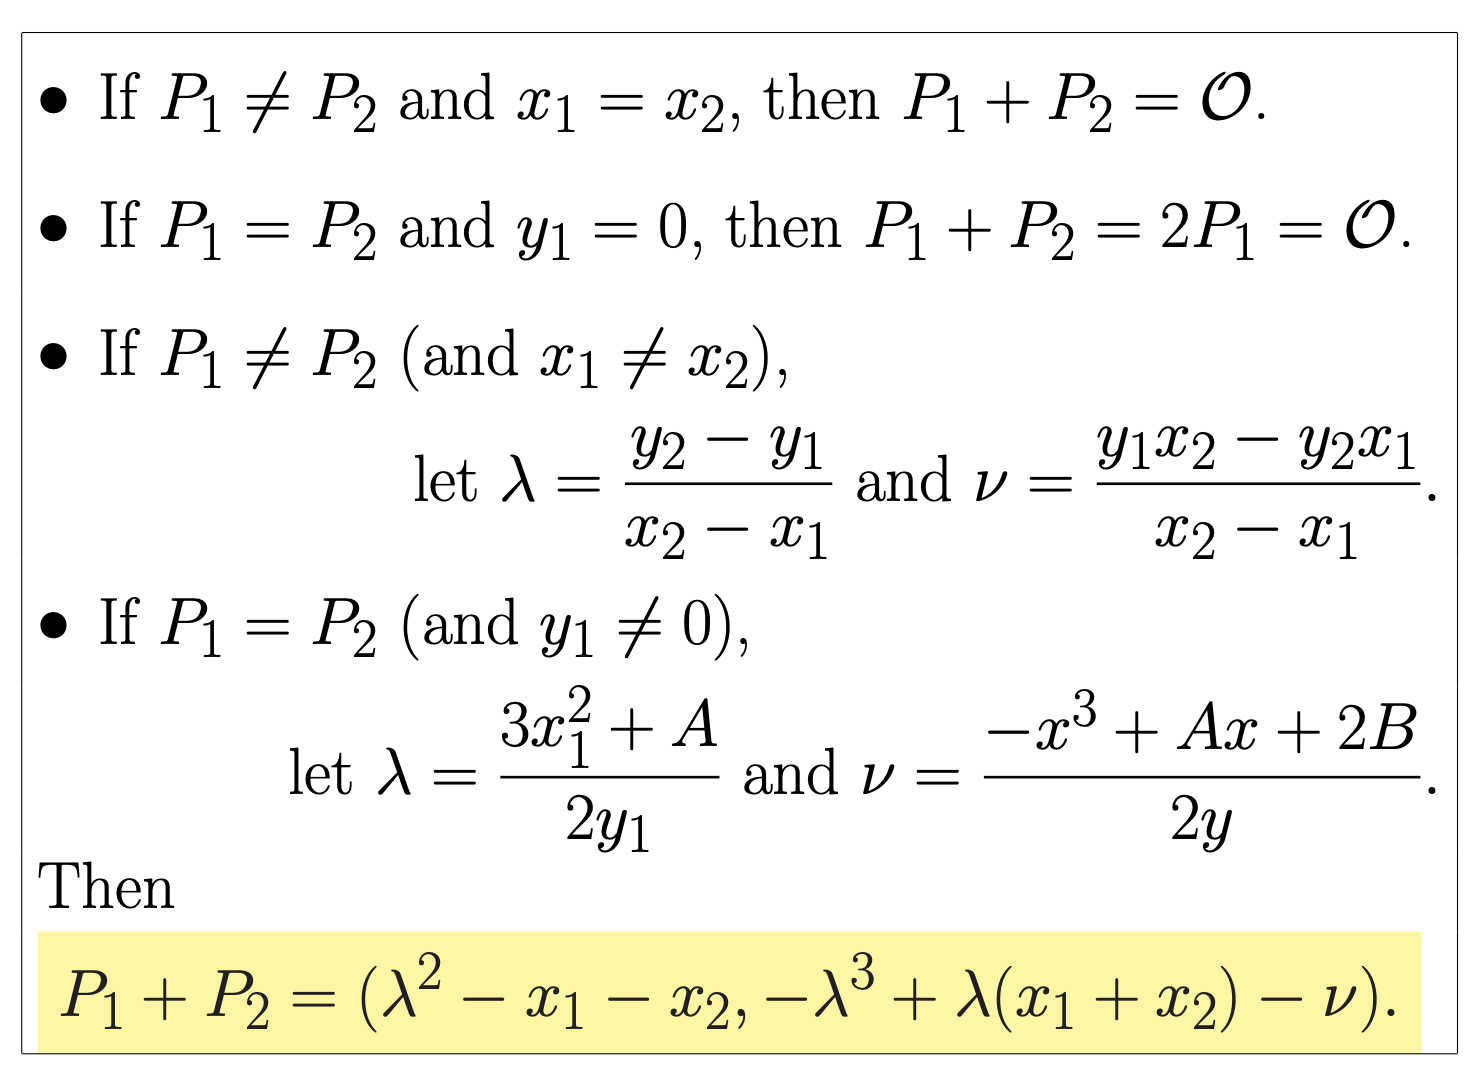
\includegraphics[width=0.85\textwidth]{Tip}
  \end{figure}

  \clearpage

  \begin{itemize}
    \item $P = (0, 1)$
    \item $P + P$
      \begin{MultiLineEquation*}{3}
          \lambda
            = \frac{3(0)^2 + 1}{2(1)}  
            = \frac{1}{2} \mod{77}    
            = 39     
      \end{MultiLineEquation*}
      \begin{MultiLineEquation*}{3}
        x
          = (39)^2 - 2(0)  \mod{77}  
          = 58 
      \end{MultiLineEquation*}
      \begin{MultiLineEquation*}{3}
        y
          = 39(0 - 58) - 1  \mod{77} 
          = 47 
      \end{MultiLineEquation*}

      Por lo tanto es $(58, 47)$

    \item $2P + P$
      \begin{MultiLineEquation*}{3}
          \lambda
            = \frac{1 -47}{0 - 58}  
            = \frac{23}{29} \mod{77}    
            = 30     
      \end{MultiLineEquation*}
      \begin{MultiLineEquation*}{3}
        x
          = (30)^2 - 58  \mod{77}  
          = 72
      \end{MultiLineEquation*}
      \begin{MultiLineEquation*}{3}
        y
          = 30(58 -72) - 47 \mod{77} 
          = 72 
      \end{MultiLineEquation*}

      Por lo tanto es $(72, 72)$

    \item $2P + 2P$
      \begin{MultiLineEquation*}{3}
        \lambda
          = \frac{3(58)^2 + 1}{2(47)}  
          = \frac{10093}{94} \mod{77}    
          = 68 * 10093  \mod{77}    
          = 23     
      \end{MultiLineEquation*}
      \begin{MultiLineEquation*}{3}
        x
          = (23)^2 - 2(58)  \mod{77}  
          = 28
      \end{MultiLineEquation*}
      \begin{MultiLineEquation*}{3}
        y
          = 23 + 23(58 * 2) - 47 \mod{77} 
          = 27
      \end{MultiLineEquation*}

      Por lo tanto es $(28, 27)$
    
      \item $4P + P$
      \begin{MultiLineEquation*}{3}
          \lambda
            = \frac{1 -27}{0 - 28}  
            = \frac{26}{28} \mod{77}    
      \end{MultiLineEquation*}

      Ahora encontramos un problema porque
      el $gcd(28, 77) \neq 1$, sino es 7, 
      y por lo mismo no podemos sumar hasta llegar
      a $5P$, pero mas importante, ya encontramos
      un factor de 77, el 7.

  \end{itemize}
      


\chapter{Tercera sección}

  Sea la curva $y^2 = x^3 + 13x + 16$ en $\Integers_{17}$

  \begin{itemize}
    \item Mostremos todos los puntos de $E$.
    
      \begin{figure}[h]
        \centering
        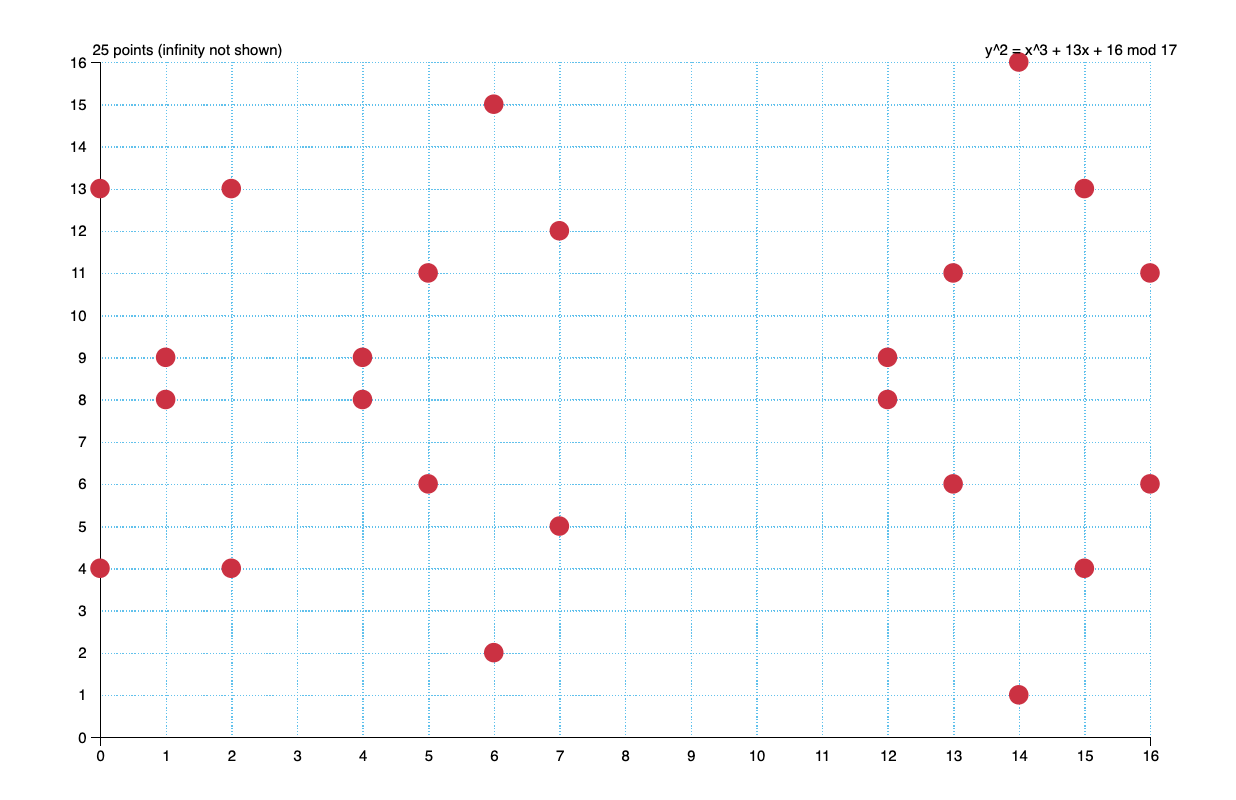
\includegraphics[width=0.55\textwidth]{3P1}
      \end{figure}

      \begin{figure}[h]
        \centering
        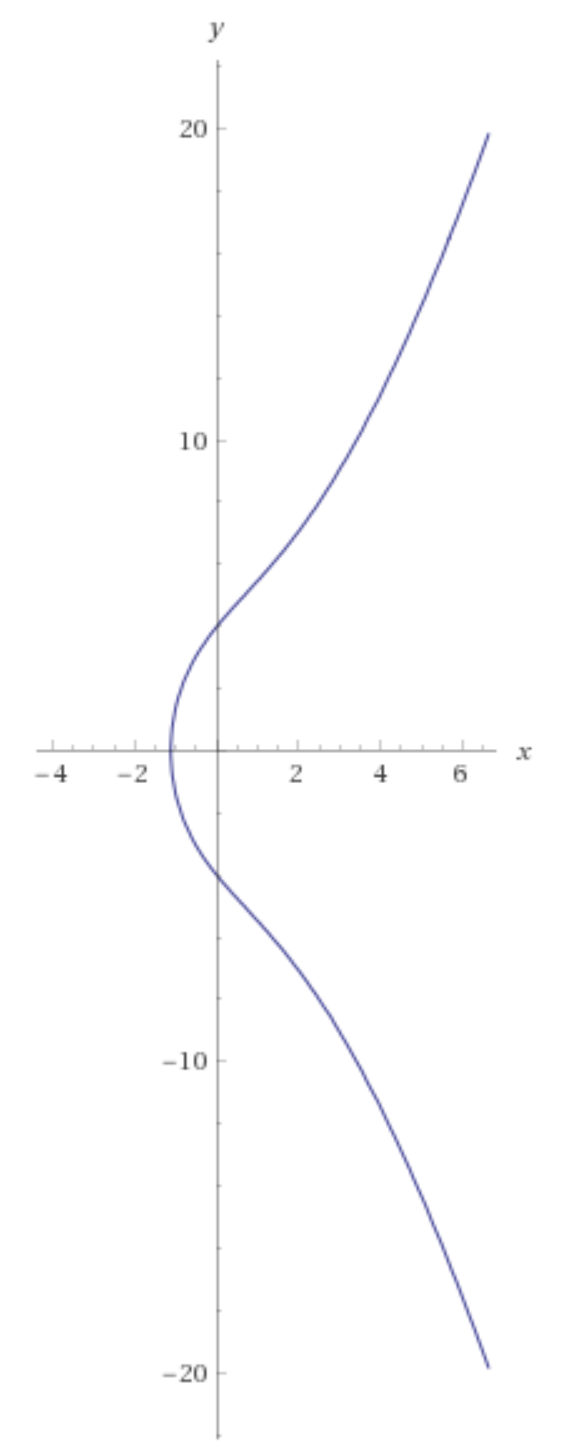
\includegraphics[width=0.15\textwidth]{3P2}
      \end{figure}
    
      Para empezar podemos hacer un programa que los calcule a todos
      por fuerza bruta, comprobando la ecuacion, con ello obtenemos
      24 puntos.

      \lstinputlisting[language=python, gobble=6]{points.py}

      Con los puntos:
      \begin{lstlisting}[gobble=8]
        [
          (0, 4), (0, 13), (1, 8), (1, 9), (2, 4), 
          (2, 13), (4, 8), (4, 9), (5, 6), (5, 11), 
          (6, 2), (6, 15), (7, 5), (7, 12), (12, 8), 
          (12, 9), (13, 6), (13, 11), (14, 1), (14, 16), 
          (15, 4), (15, 13), (16, 6), (16, 11)
        ]
      \end{lstlisting}

      Siendo mas formales por definicion se consideran 
      los puntos como:
      
      $E(L) 
        = \Set{\infty} u \Set{ (x, y) \in L \times L | 
        y^2 = x^3 + 13x + 16}$

      Es decir los puntos del programa mas el infinito.

    \item 
      Alicia desea enviar el siguiente mensaje 
      $C = (a, b) = ((6, 2),(14, 1))$ a Bob, los parametros
      publicos de Bob son $\alpha = (0, 13) \in E$ una raiz 
      primitiva y $\beta = (15, 13)$, donde $beta = s\alpha$ 
      y $s$ su llave privada. 
      
      Usa cualquier algoritmo mencionado en la seccion 5.2 
      del libro Elliptic Curves Number Theory and Cryptography 
      de Lawrence C. Washington Para resolver logaritmo.


      Vamos a hacer el algoritmo de Paso chico, paso grande.

      Ya sabemos el orden del grupo (25), lo que podemos seleccionar
      a $m = 6$, pues $m \geq \sqrt{N}$.

      Ahora podemos computar $mP =  6(0, 13)$, esto va vimos como hacerlo a mano,
      así que solo mostraremos el resultado final:

      \begin{itemize}
        \item $2(0, 13) = (13, 6)$
        \item $3(0, 13) = (6, 2)$
        \item $4(0, 13) = (12, 9)$
        \item $5(0, 13) = (7, 12)$
        \item $6(0, 13) = (1, 9)$
      \end{itemize}

      Ahora tenemos que hacer lo siquiente:
     \begin{SmallIndentation}[0.7em]
      \begin{itemize}
        \item $Q - jmP 
          = (15, 13) - 1(1, 9)
          = (15, 13) + (1, 8)
          = (0, 13)
          $
        \item $Q - jmP 
          = (15, 13) - 2(1, 9)
          = (15, 13) - (16, 6)
          = (15, 13) + (16, 11)
          = (7, 5)
          $
        \item $Q - jmP 
          = (15, 13) - 3(1, 9)
          = (15, 13) - (15, 14)
          = (15, 13) + (15, 3)
          = (0, 0)
          $
        \item $Q - jmP 
          = (15, 13) - 4(1, 9)
          = (15, 13) - (0, 4)
          = (15, 13) + (0, 13)
          = (2, 4)
          $
        \item $Q - jmP 
          = (15, 13) - 5(1, 9)
          = (15, 13) - (7, 12)
          = (15, 13) + (7, 5)
          = (13, 6)
          $
        \item $Q - jmP 
          = (15, 13) - 6(1, 9)
          = (15, 13) - (5, 6)
          = (15, 13) + (5, 11)
          = (12, 8)
          $
      \end{itemize}
    \end{SmallIndentation}

      Y es aqui cuando me di por vencido, luchando, hasta que me di cuenta que se
      me habia olvidado lo mas obvio:
      $1(0, 13) = (0, 13)$.

      Y mira que:
      $Q - jmP 
          = (15, 13) - 1(1, 9)
          = (15, 13) + (1, 8)
          = (0, 13)
          $

      Por lo tanto podemos ver que:
      $iP = Q - jmP$, por lo tanto la respuesta es $i + jm \mod{N}$, 
      es decir $1 + 1(6) \mod{N} = 7$.

      Y mira que estuve muy cerca de calcularla.

      Por lo tanto $7(0, 13) = (15, 13)$

  \item 
    A partir de la informacion encontrada antes descifra el mensaje enviado a Bob
    
    Solucion: Usando ElGamal (pagina 188 del libro) siguiendo la formula de:
      $M = M2 - sM1$

      Se tiene que:
      \begin{MultiLineEquation*}{3}
      M 
        &= (14, 1)  -s  (6, 2)  \\
        &= (14, 1)  -7  (6, 2)  \\
        &= (14, 1)   -   (12, 8) \\
        &= (14, 1)  +   (12, 9) \\
        &= (7, 5)
      \end{MultiLineEquation*}

      Donde el mensaje original es $M = (7, 5)$.

  \end{itemize}


  \chapter{Cuarta sección}

  Sea la curva $y^2 = x^3 + 7x + 19$ en $\Integers_{31}$ y $P = (18, 26)$ un punto en E 
  de orden 39, el ECIES simplificado definido sobre $\Integers_{31}$
  como espacio de texto plano, supongamos que la clave privada es $m = 8$.

  \begin{itemize}
    \item 
      Usando lo que vimos antes podemos solo mostrar el resultado:

      $Q = mP = 8(18, 26) = (10, 2)$

    \item 
    Descifra la siguiente cadena de texto cifrado: \\
      $((4, 1), 1); ((11, 0), 18); ((27, 1), 17); ((28, 1), 29); ((23, 0), 26)$

      Sabemos que en el criptosistem ECIES simplificado, el mensaje cifrado es de la
      forma $((Zp \times Z_2) \times Zp^*) = (y_1, y_2)$

      Como el orden de P es el mismo que E, P es un generador y puede ser usado en la
      encriptacion de ECIES simplificado.

      Los puntos de compresion recibidos son:
      $(4,1), (11,0), (27,1), (28,1), (23,0)$
      
      Debemos calcular sus respectivos puntos de descompresion.
      Sabemos que:
      
      $z \leftarrow (x^3 + 7x + 19)  \mod{31}$

      \begin{itemize}
        \item 
          \begin{MultiLineEquation*}{3}
            z
            \leftarrow (x^3 + 7x + 19)  \mod{31}        \\
            \leftarrow (4^3 + 7(4) + 19)  \mod{31}       \\
            \leftarrow 111  \mod{31}        \\
            \leftarrow 18  \mod{31}
          \end{MultiLineEquation*}

          Por lo que $y = \pm 7$, por la segunda componentes es $y = 7$.
          por lo tanto el punto es $8 * (4, 7) = (2, 17)$.

          $d = 1 * 2^{-1} \mod {31} = 16 = 16 \mod{31}$, 
          es decir $P$.

        \item 
          \begin{MultiLineEquation*}{3}
            z
            \leftarrow (x^3 + 7x + 19)  \mod{31}       \\
            \leftarrow (11^3 + 7(11) + 19)  \mod{31}       \\
            \leftarrow 1427  \mod{31}       \\
            \leftarrow 1  \mod{31}
          \end{MultiLineEquation*}

          Por lo que $y = \pm 1$, por la segunda componentes es $y = 30$.
          por lo tanto el punto es $8 * (11, 30) = (23, 3)$.

          $d = 18 * 23^{-1} \mod {31} = 18 * 27 = 21 \mod{31}$, 
          es decir $U$.

        \item 
          \begin{MultiLineEquation*}{3}
            z
            \leftarrow (x^3 + 7x + 19)  \mod{31}       \\
            \leftarrow (27^3 + 7(27) + 19)  \mod{31}       \\
            \leftarrow 19 891  \mod{31}       \\
            \leftarrow 20  \mod{31}
          \end{MultiLineEquation*}

          Por lo que $y = \pm 12$, por la segunda componentes es $y = 19$.
          por lo tanto el punto es $8 * (27, 19) = (18, 26)$.

          $d = 17 * 18^{-1} \mod {31} = 17 * 19 = 13 \mod{31}$, 
          es decir $M$.
      
        \item 
          \begin{MultiLineEquation*}{3}
            z
            \leftarrow (x^3 + 7x + 19)  \mod{31}        \\
            \leftarrow (28^3 + 7(28) + 19)  \mod{31}       \\
            \leftarrow 22 167  \mod{31}       \\
            \leftarrow 2  \mod{31}
          \end{MultiLineEquation*}

          Por lo que $y = \pm 2$, por la segunda componentes es $y = 23$.
          por lo tanto el punto es $8 * (28, 23) = (29, 20)$.

          $d = 29 * 29^{-1} \mod {31} = 1 \mod{31}$, 
          es decir $B$.
      

      \item 
        \begin{MultiLineEquation*}{3}
          z
          \leftarrow (x^3 + 7x + 19)  \mod{31}        \\
          \leftarrow (23^3 + 7(23) + 19)  \mod{31}        \\
          \leftarrow 12 347  \mod{31}       \\
          \leftarrow 9  \mod{31}
        \end{MultiLineEquation*}

        Por lo que $y = \pm 3$, por la segunda componentes es $y = 28$.
        por lo tanto el punto es $8 * (23, 28) = (3, 25)$.

        $d = 26 * 3^{-1} \mod {31} = 26 * 21 = 19 \mod{31}$, 
        es decir $S$.

        Por lo mismo el mensaje oculto es:
        PUMBS
      \end{itemize}

      

      
      

      

  
  
  \end{itemize}


  \begin{thebibliography}{10}

    \bibitem{Menezes} 
      Alfred J. Menezes, Scott A. Vanstone, and Paul C. Van Oorschot. 1996. Handbook of Applied
      Cryptography (1st ed.). CRC Press, Inc., Boca Raton, FL, USA.

  \end{thebibliography}



\end{document}